%%%%%%%%%%%%%%%%%%%%%%%%%%%%%%%%%%%%%%%%%%

\chapter{Demonstration of simultaneous spin analyzer}\label{chap:ssa_2020}

%%%%%%%%%%%%%%%%%%%%%%%%%%%%%%%%%%%%%%%%%%

We present spin asymmetry measurements taken in 2020 using an early iteration of the simultaneous spin analyzer (\acrshort{ssa}) and the improvements applied to the apparatus in light of the results.

%%%%%%%%%%%%%%%%%%%%%%%%%%%%%%%%%%%%%%%%%%

\section{Description of apparatus (2020)}

%%%%%%%%%%%%%%%%%%%%%%%%%%%%%%%%%%%%%%%%%%

\begin{figure}[hbp]
    \centering
    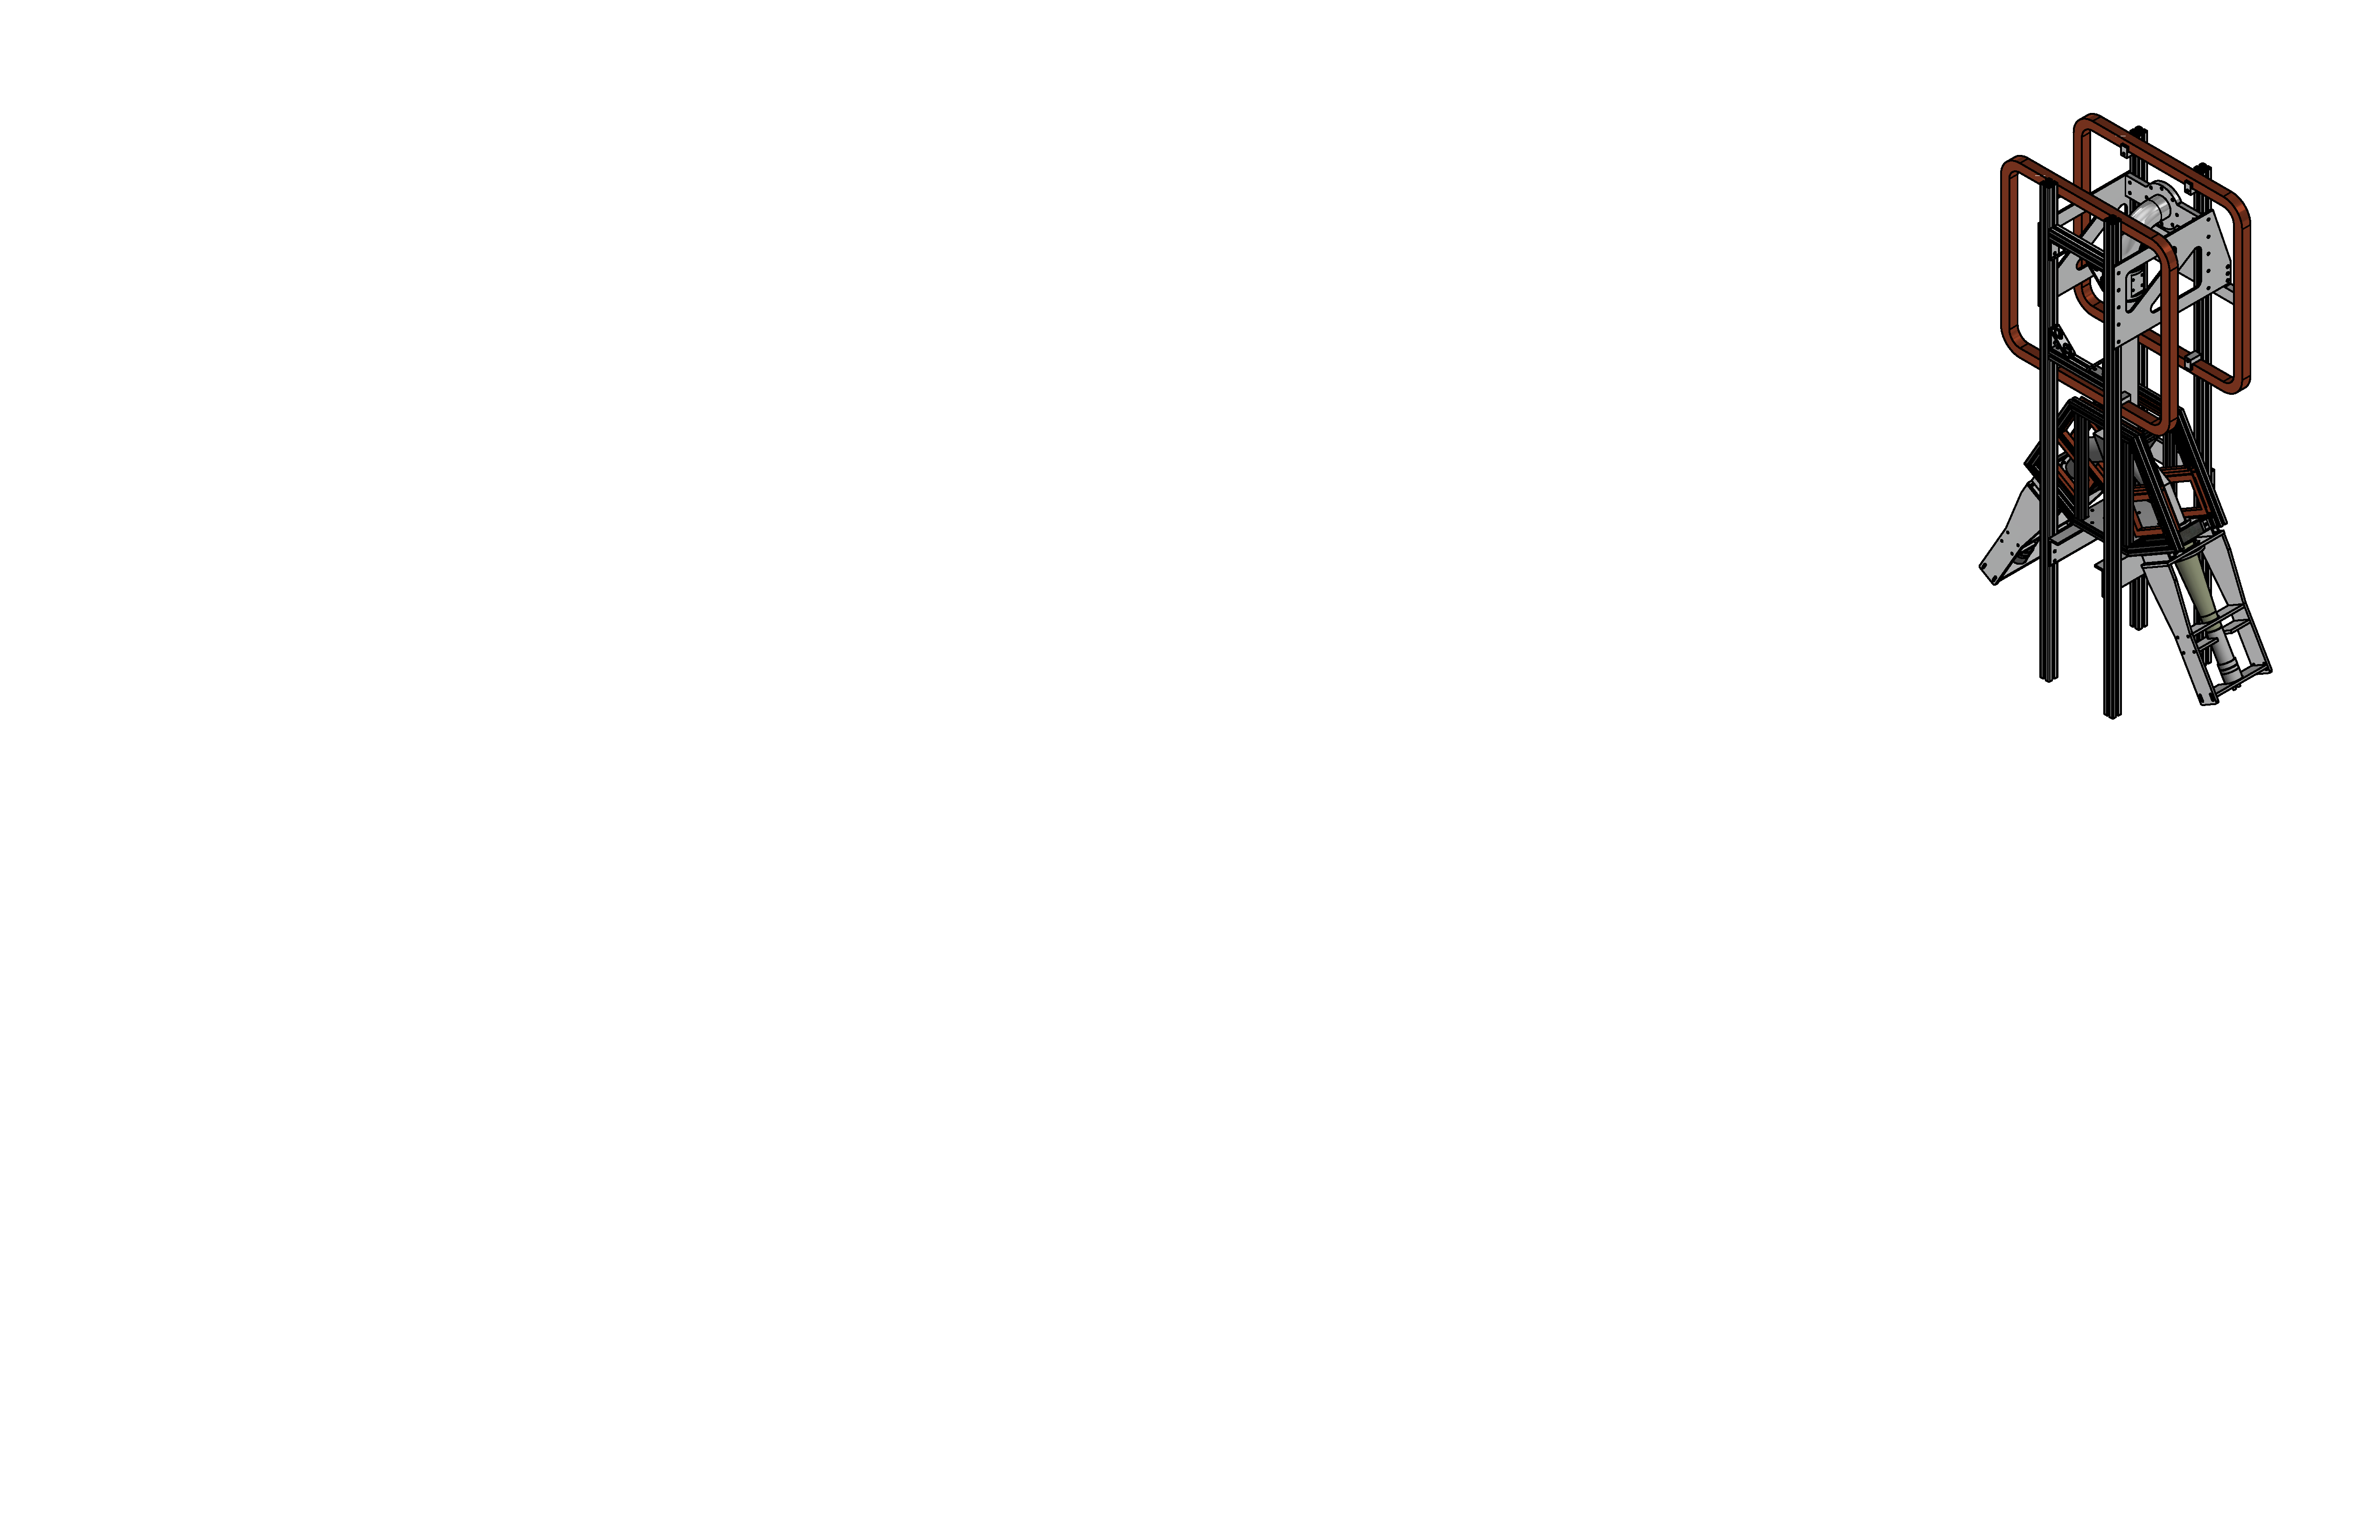
\includegraphics[height=3.1in]{figures/ssa_schematic_colorized.pdf}
    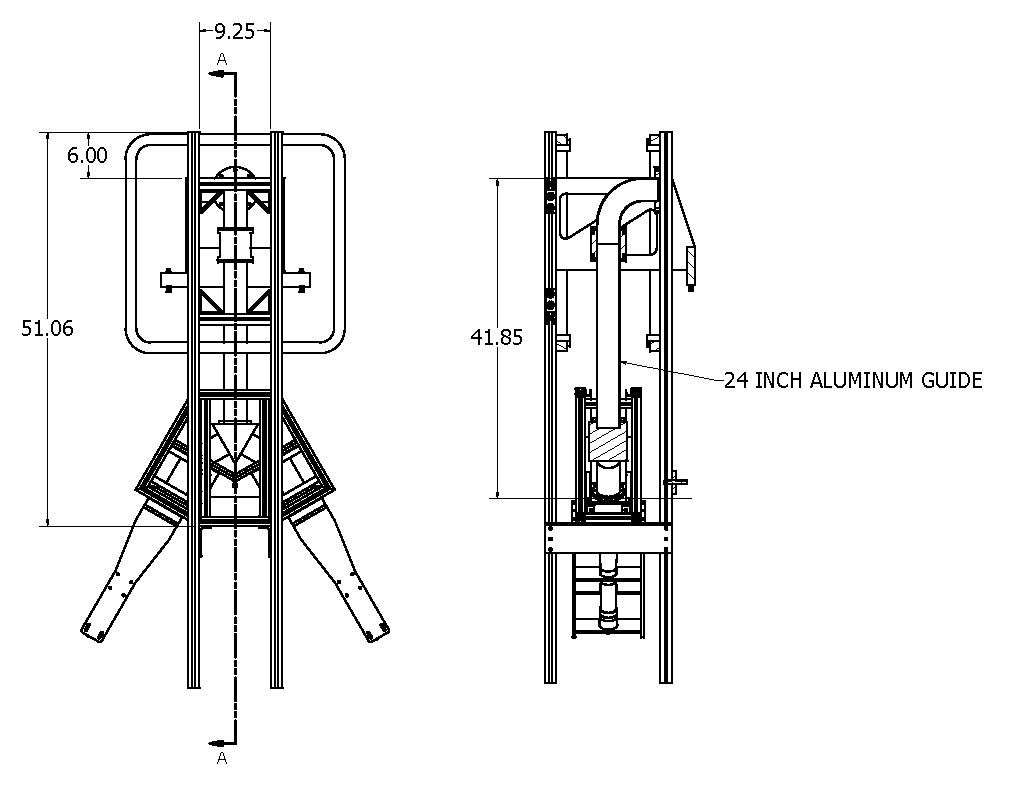
\includegraphics[height=3.5in]{figures/ssa_schematics.pdf}
    \caption
    {Schematics for first iteration of simultaneous spin analyzer, mounting frame, and associated transport coils. Courtesy of Mark Luxnat.}
    \label{fig:ssa_schematic}
\end{figure}

The SSA was mounted to the rotary switcher on the Chap.~\ref{chap:north_beamline_paper} North beamline setup (Fig.~\ref{sec:northBeamlineSetup}) on the port opposite to the drop detector. As in Fig.~\ref{fig:ssa_schematic}, a \qty{90}{\degree} bend connected to the switcher was extended downwards by a \qty{24}{in} NiP-coated Al guide. The bottom of the Al guide was connected to a wye comprised of NiMo-coated glass. Each arm of the SSA wye contained the same spin flipper, polarizer, \BZnS scintillator, and iron yoke flux return design as the drop detector (Sec.~\ref{sec:spin_flipper_analyzer}). The neutron guides were kept under a  $\sim \qty{1}{mT}$ field by coils.


%%%%%%%%%%%%%%%%%%%%%%%%%%%%%%%%%%%%%%%%%%

\section{Measurements}\label{sec:ssa_measurements}

%%%%%%%%%%%%%%%%%%%%%%%%%%%%%%%%%%%%%%%%%%

\begin{table}
\centering
\caption
{Beam parameters at the LANL accelerator for reduction of beam current to $\sim \qty{1}{\micro A}$ (nominal $\sim \qty{10}{\micro A}$), as used in flow-through \ucn measurements}\label{tb:flow_through_beam_params}
\begin{tabular}{ll}
\toprule
Parameter & Setting \\
\midrule
Capture HG\textminus X & 77\% \\
Countdown & 1 (8 nominal) \\
Patter width & 327 \\
Pulses per burst & 9 \\
Time between bursts & \qty{4.975}{s} \\
\bottomrule
\end{tabular}
\end{table}

To perform an asymmetry measurement, \ucn were in continuous flow-through mode from the source to the spin analyzer(s), while the RF spin flipper frequency was swept.  The integrated counts from the detector for each period were normalized to the West GV monitor as per Sec.~\ref{subsec:dataProcessing}. As discussed in Sec.~\ref{sec:north_beamline_discussion}, the continuous use of the UCN source alters the input energy spectrum into the experiment~\cite{anghel_solid_2018}. To limit the impact of the flow-through mode measurements on the source, the beam current was reduced by a factor of 10 to $\sim \qty{1}{\micro A}$. Adjusted beam parameters are listed in Tab.~\ref{tb:flow_through_beam_params}.

As a benchmark, the asymmetry measurement was first performed on the drop detector. The RF frequency was incremented every \qty{10}{s}, but to allow the UCN rate to stabilize only the middle \qty{7}{s} of each toggle was considered a counting period. Figure~\ref{fig:spin_flipper_efficiency} depicts the normalized \ucn counts at each frequency step as a fraction of the baseline (RF coil off). 

For the SSA asymmetry measurement, the North GV was toggled on and off every 30 seconds, which allowed neutrons in the guide system to fully drain into the detector. The spin flipper frequency was only incremented prior the the opening of the North GV. This was then repeated for each arm of the SSA. Unlike the drop detector, the SSA did not yet have an impedance matching circuit. To compensate, the RF coils were driven by a SRS DS345 function generator, with an amplifier that gave a factor of 7 to 9 times gain. An input peak-to-peak amplitude of \qty{1}{V} gave an $\sim\qty{7}{V}$ signal after the amplifier, and an input of \qty{1.8}{V} gave an output of $\sim\qty{18}{V}$.

Figures~\ref{fig:Fall2020_SSA_RF_east} and \ref{fig:Fall2020_SSA_RF_west} depict the  normalized \ucn counts at each frequency step as a fraction of the baseline for each SSA arm (arbitrarily named ``East'' and ``West''). The flow-through measurement was also repeated for each arm with the polarizing foil on the opposing arm removed (Fig.~\ref{fig:SSA_asym_one_foil_out}).





\begin{figure}
    \centering
    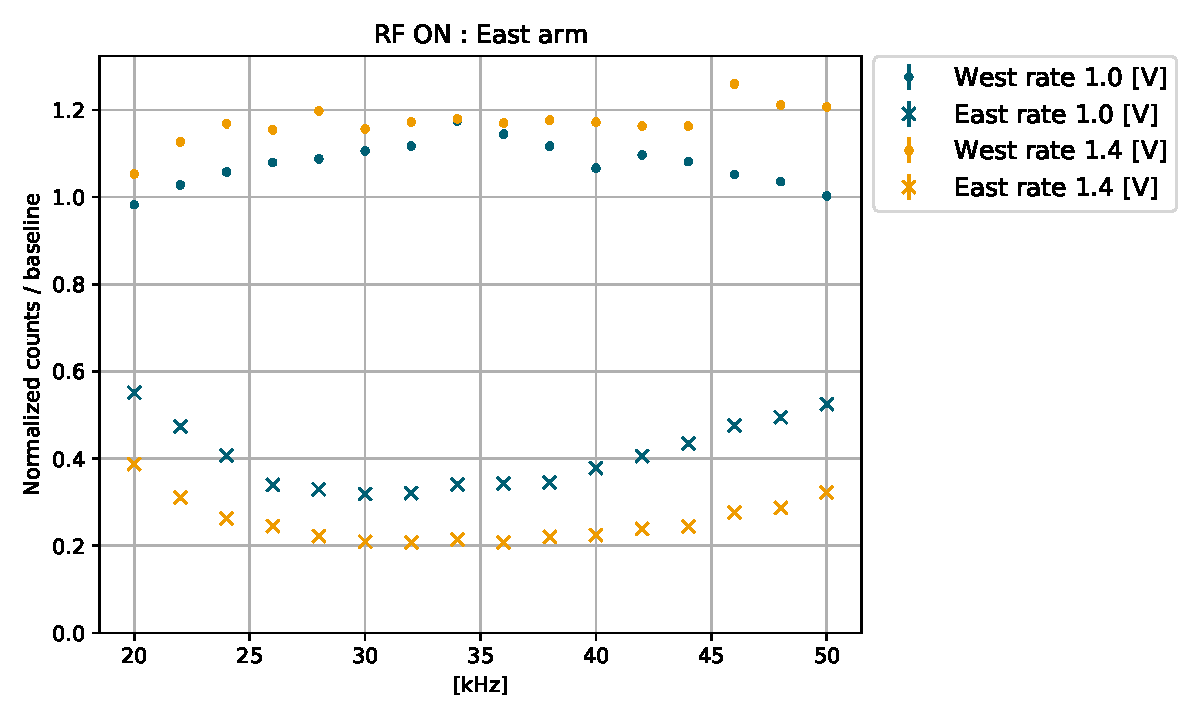
\includegraphics[width=0.7\textwidth]{figures/RF_ON_East_arm.pdf}
    \caption
    [Flow through measurement of UCN from the source to the simultaneous spin analyzer, with the RF spin flipper on the ``East'' arm energized.]
    {Flow through measurement of UCN from the source to the simultaneous spin analyzer, with the RF spin flipper on the ``East'' arm energized. Measurements for various peak-to-peak RF amplitudes (before amplification, c.f. Sec.~\ref{sec:ssa_measurements}). Normalized detector counts on the $y$-axis are depicted as a fraction of the respective detector's baseline count rate with the RF spin flipper off. Error bars are smaller than the markers}
    \label{fig:Fall2020_SSA_RF_east}
% \end{figure}
    \vspace{\baselineskip}
% \begin{figure}
    \centering
    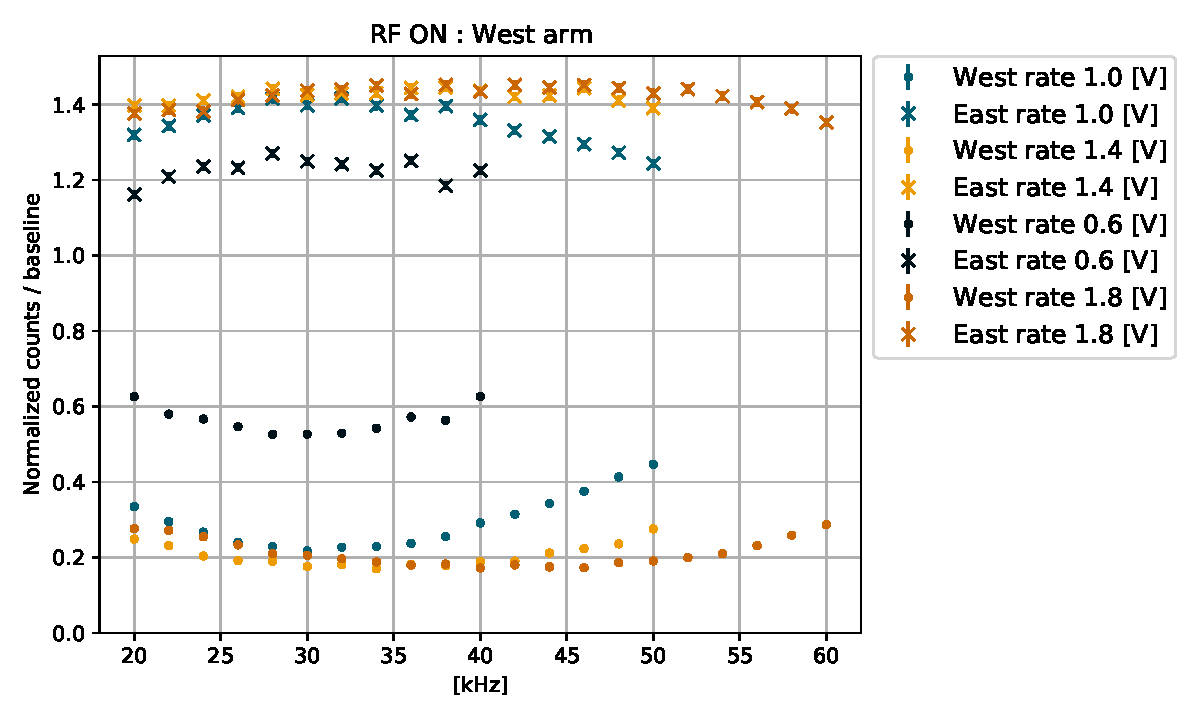
\includegraphics[width=0.7\textwidth]{figures/RF_ON_West_arm.pdf}
    \caption
    [Flow through measurement of UCN from the source to the simultaneous spin analyzer, with the RF spin flipper on the ``West'' arm energized.]
    {Flow through measurement of UCN from the source to the simultaneous spin analyzer, with the RF spin flipper on the ``West'' arm energized. Error bars are smaller than the markers.}\label{fig:Fall2020_SSA_RF_west}
\end{figure}

\begin{figure}
\centering
%subfigure width gets "multiplied" by includegraphics width
\begin{subfigure}{.5\textwidth} 
  \centering
  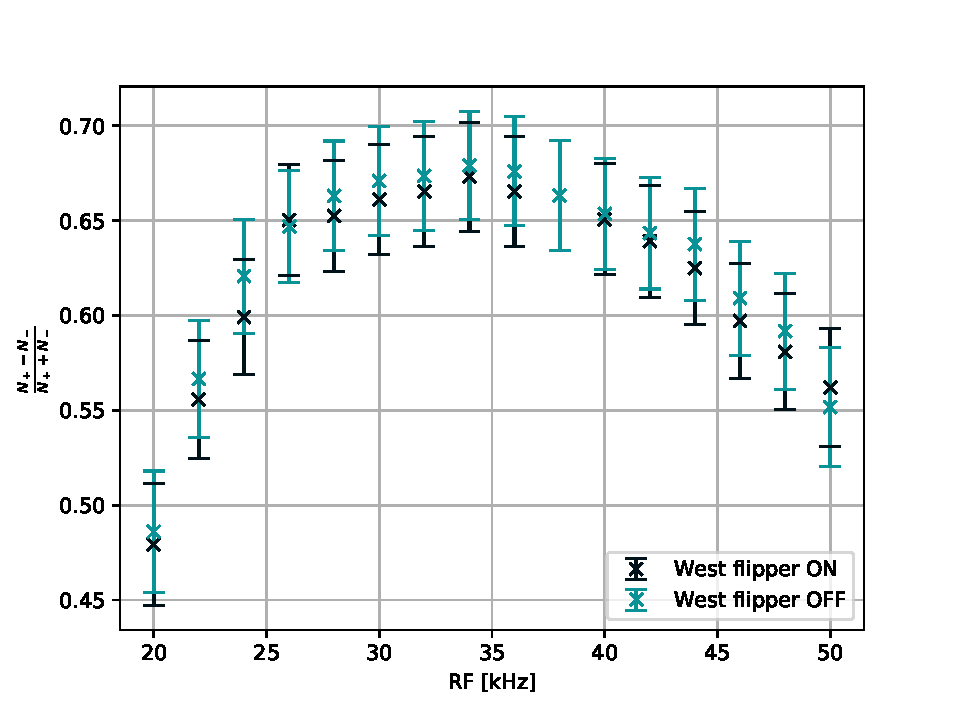
\includegraphics[width=\textwidth]{figures/SSA_east_arm_no_west_foil.pdf}
  \caption{East arm asymmetry, no foil on West arm }\label{subfig:SSA_east_arm_no_west_foil}
\end{subfigure}%DO NOT REMOVE THIS '%'
\begin{subfigure}{.5\textwidth}
  \centering
  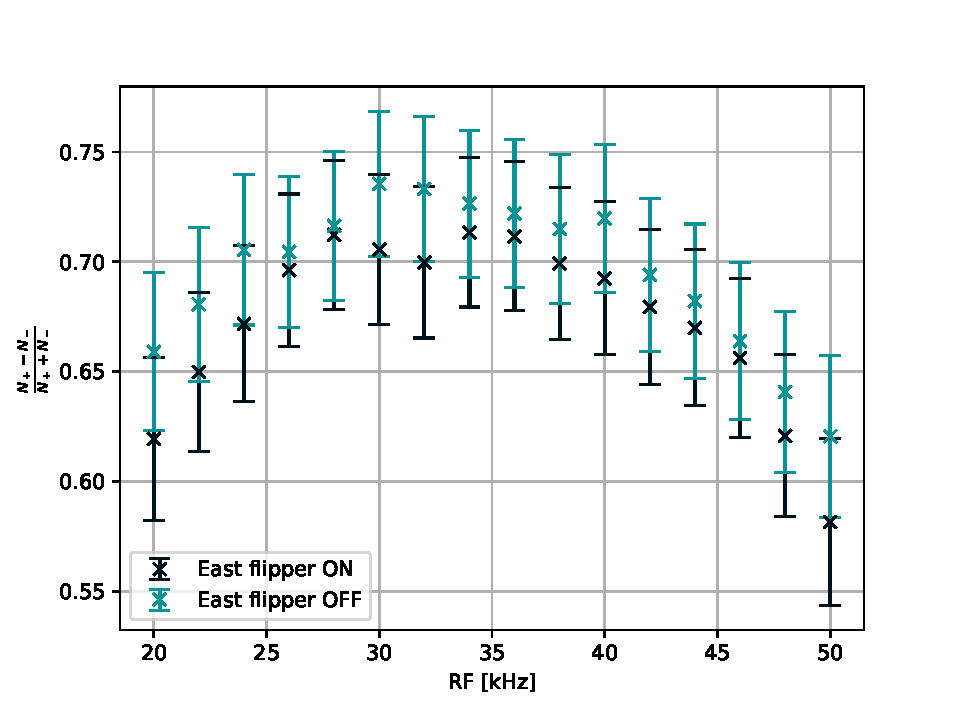
\includegraphics[width=\textwidth]{figures/SSA_west_arm_no_west_foil.pdf}
  \caption{West arm asymmetry, no foil on East arm}\label{subfig:SSA_west_arm_no_west_foil}
\end{subfigure}
\caption
    [Spin asymmetry (Eq.~(\ref{eq:spin_asymmetry})) measurement in one arm of the simultaneous spin analyzer, with the polarizing foil on the opposite arm removed.]
    {Spin asymmetry (Eq.~(\ref{eq:spin_asymmetry})) measurement in one arm of the simultaneous spin analyzer, with the polarizing foil on the opposite arm removed. ($V_\text{pp, in}=\qty{1.4}{V}$). As validation, the measurement was repeated with the RF coil on/off in the arm without the polarizer, with the expectation that the asymmetry should be equivalent.}
\label{fig:SSA_asym_one_foil_out}
\end{figure}

%%%%%%%%%%%%%%%%%%%%%%%%%%%%%%%%%%%%%%%%%%

\section{Discussion}

%%%%%%%%%%%%%%%%%%%%%%%%%%%%%%%%%%%%%%%%%%

We first compare asymmetry (calculated with Eq.~(\ref{eq:spin_asymmetry})) between the drop detector and each of the SSA arms. From Fig~\ref{fig:spin_flipper_efficiency}, when the RF coil is at the \qty{20}{kHz} resonant frequency the neutron count drops to 12\% of the baseline. The asymmetry for the drop detector is then $A\approx 0.8$. For the ``East'' arm (Fig.~\ref{fig:Fall2020_SSA_RF_east}), the input amplitude of \qty{1.4}{V} at the \qty{34}{kHz} resonance reduces neutron counts to 21\% of the baseline ($A=0.65(3)$). For the ``West'' arm (Fig.~\ref{fig:Fall2020_SSA_RF_west}) the same resonance reduces neutron count to 17\% ($A=0.69(3)$). 

While both SSA arms exhibited comparable spin asymmetry, they were outperformed by the single analyzer system. To rule out the possibility of SSA guide segments being spin-depolarizing, the \qty{90}{\degree} bend was replaced with a spare component, but the asymmetry measurements at resonance were not significantly altered.

From Figs.~\ref{fig:Fall2020_SSA_RF_east}--\ref{fig:Fall2020_SSA_RF_west}, it can be seen that that as spin flipped neutrons were rejected on one arm, the other arm measured increased counts. It was then postulated that if the NiMo wye was depolarizing, repeated \ucn bounces between both arms of the SSA could result in worse asymmetry. This led to the measurement in Fig.~\ref{fig:SSA_asym_one_foil_out}, where the foil on the opposing arm was removed to limit cross-talk between the arms. As validation, the measurement was repeated with the RF coil on/off in the arm without the foil, with the expectation that the asymmetry should be equivalent. At \qty{34}{kHz}, the East arm had $A=0.68(3)$ and the West arm had $A=0.73(3)$, which was not a statistically meaningful change from the asymmetry measurement with both foils installed.

Again examining the resonant peak of Fig.~\ref{fig:spin_flipper_efficiency}, the SSA resonance peaks in Figs.~\ref{fig:Fall2020_SSA_RF_east}--\ref{fig:Fall2020_SSA_RF_west} were significantly wider in comparison. This implies that for the SSA there was a larger gradient in the static magnetic field $B_\text{stat}$ in the region of the RF spin flippers. From Eq.~(\ref{eq:adiab_derivation_1}), the resonant frequency for spin flipping is $\gls{gamma_n} B_\text{stat}$. For a widely varying $B_\text{stat}$ the range of frequencies for optimized adiabatic spin flipping increases.

To confirm the magnetic field gradient, an in-situ magnetic field map was attempted. When mounted on the switcher, however, accessing the spin flipping region in the wye with a Hall probe required the removal of the spin polarizing foil. Without the polarizer completing the magnetic flux ``circuit'' of the iron yoke, the magnetic field gradients from the polarizer ferromagnets could not be decoupled from the ambient gradients. Field mapping was delayed until after the 2020 measurement cycle, when the SSA was dismounted from the switcher for Hall probe access through the stem of the wye. An attempt was also made to slide the RF coils along the arms of the wye farther away from the iron yoke to a region with potentially milder gradients, but it was impeded by the presence of unnecessary aluminum sleeves enclosing the RF coils.

Another observation from the SSA tests was that non-horizontal polarizer foils (seen in Fig.~\ref{fig:ssa_schematic}) could affect measured spin asymmetry. For \ucn with a downward vertical trajectory in the SSA, the kinetic energy component $K_\perp$ perpendicular to the surface of the spin polarizer would be reduced, lowering transmission probability (Sec.~\ref{sec:ucn_reflection_transmission}). While the issue could be mitigated simply by extending the vertical guide segment and using gravity to increase $K_\perp$ (Sec.~\ref{sec:ucn_grav_em}), the SSA mounting frame at the time was unable to accommodate extensions.

\begin{figure}[htp]
    \centering
    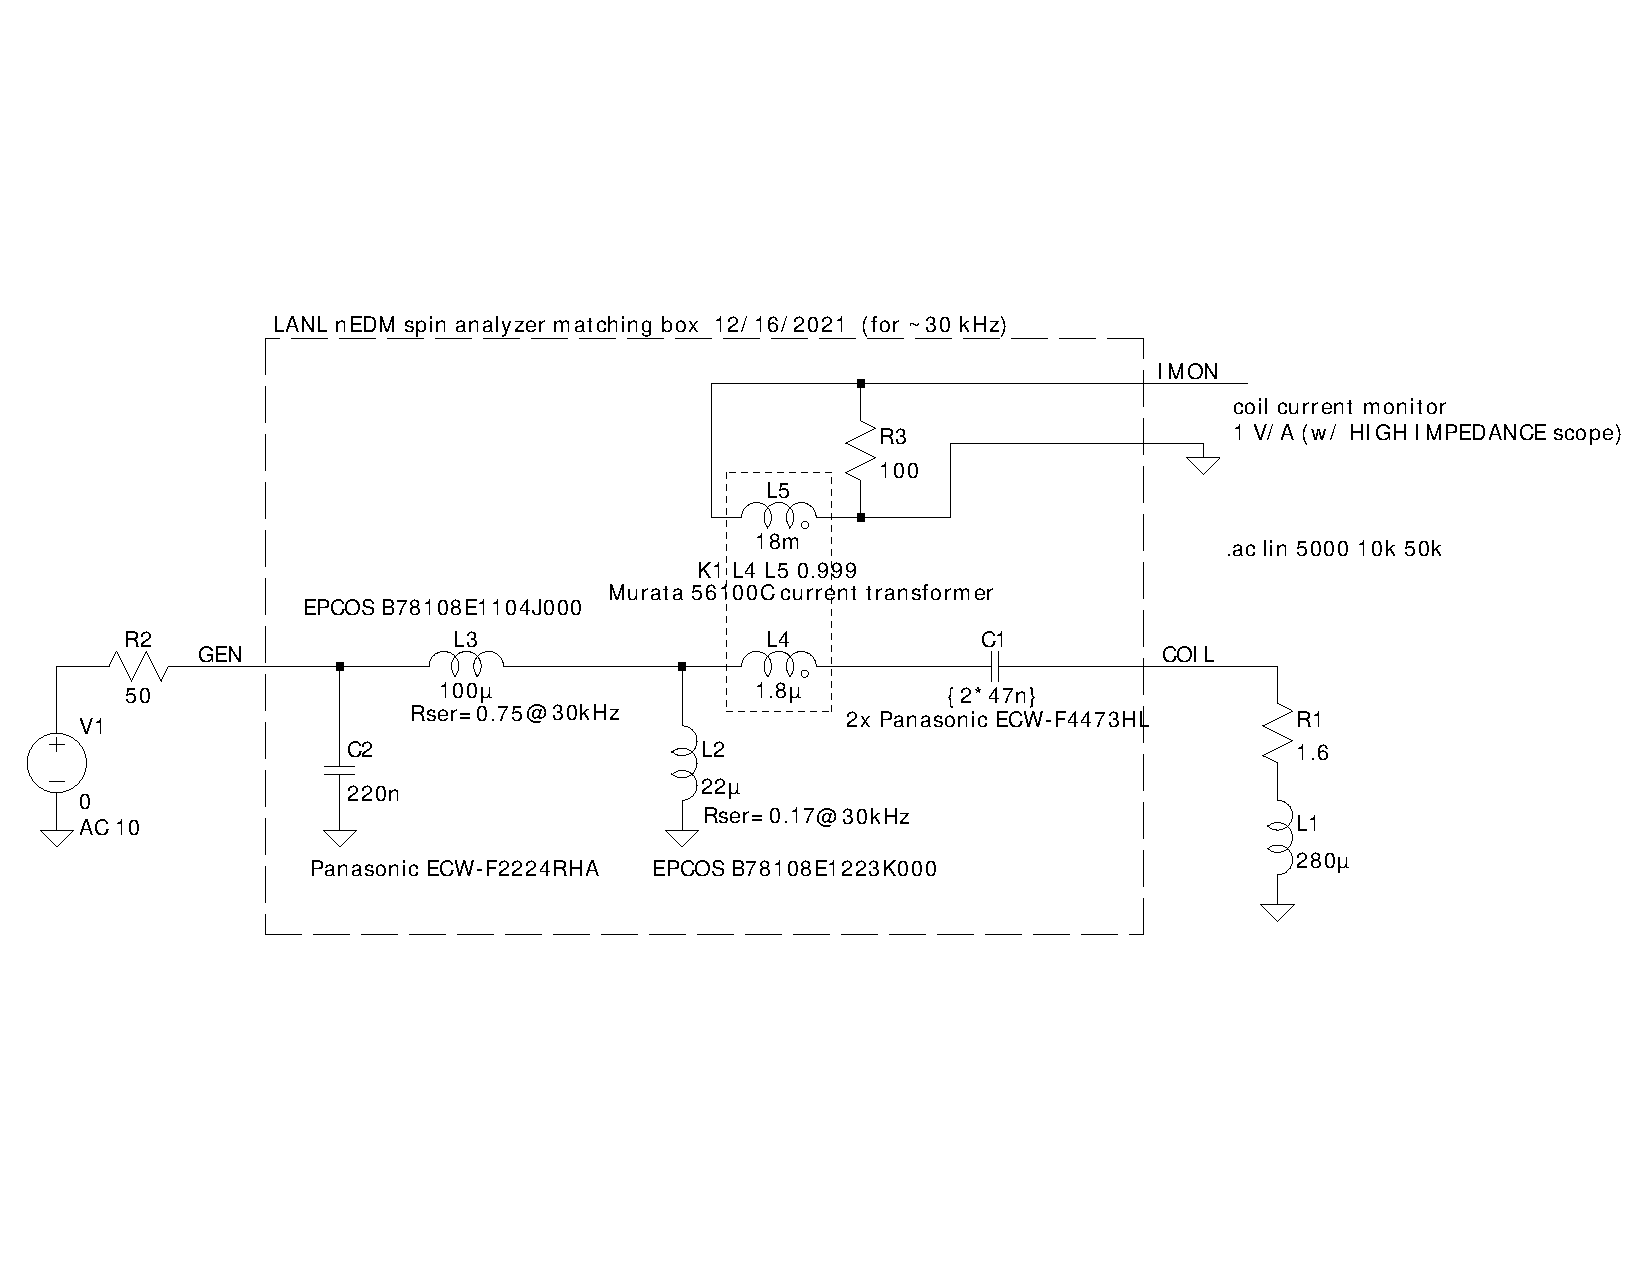
\includegraphics[width=\textwidth]{figures/matching_box_30kHz.pdf}
    \caption
    [Circuit of the impedance matching box for the simultaneous spin analyzer, designed for the nominal RF frequency of \qty{30}{kHz}.]
    {Circuit of the impedance matching box for the simultaneous spin analyzer, designed for the nominal RF frequency of \qty{30}{kHz}. Figure and matching box courtesy of Gerard Visser.}
    \label{fig:ssa_matching_box}
\end{figure}

Following the 2020 measurement cycle, the following upgrades were implemented:
%
\begin{enumerate}
    \item The SSA switcher mounting frame was extended and an additional \qty{15}{in} of vertical NiP-coated Al guide was added.
    \item The aluminum sleeves enclosing the RF coils were removed and the RF coils were placed farther from the iron yoke. The RF coils were replaced with new versions wound with thinner-gauge wire for a larger RF amplitude.
    \item The magnetic field in the region of the spin flipper was mapped with a Hall probe with the polarizer foils inserted in the flux return yoke. From the field map, a nominal RF operating frequency of \qty{30}{kHz} (corresponding to a field $B_\text{stat}=\qty{100}{\micro T}$) was determined. An impedance matching circuit (Fig.~\ref{fig:ssa_matching_box}) for the RF coils at the nominal operating frequency was then created.\label{enum:ssa_upgrade}
    \item The PMTs on the SSA were replaced with Onsemi \acrshort{sipm} 4-Side Scaleable Arrays (C Series) to avoid potential complications of the PMTs being located too close to the iron yoke ferromagnets. (The light guide on the drop detector was much longer than the the SSA light guides, so it did not share this issue)
\end{enumerate}
%
A second SSA system was also constructed with the above improvements incorporated. As per point (\ref{enum:ssa_upgrade}), future asymmetry measurements with the SSAs will avoid adjusting the nominal RF coil frequency, and instead sweep the strength of the holding field coals in the spin flipper region.


